\section{Mode FSM}
  \begin{frame}{mode FSM Interface}  
  	\begin{figure}
  		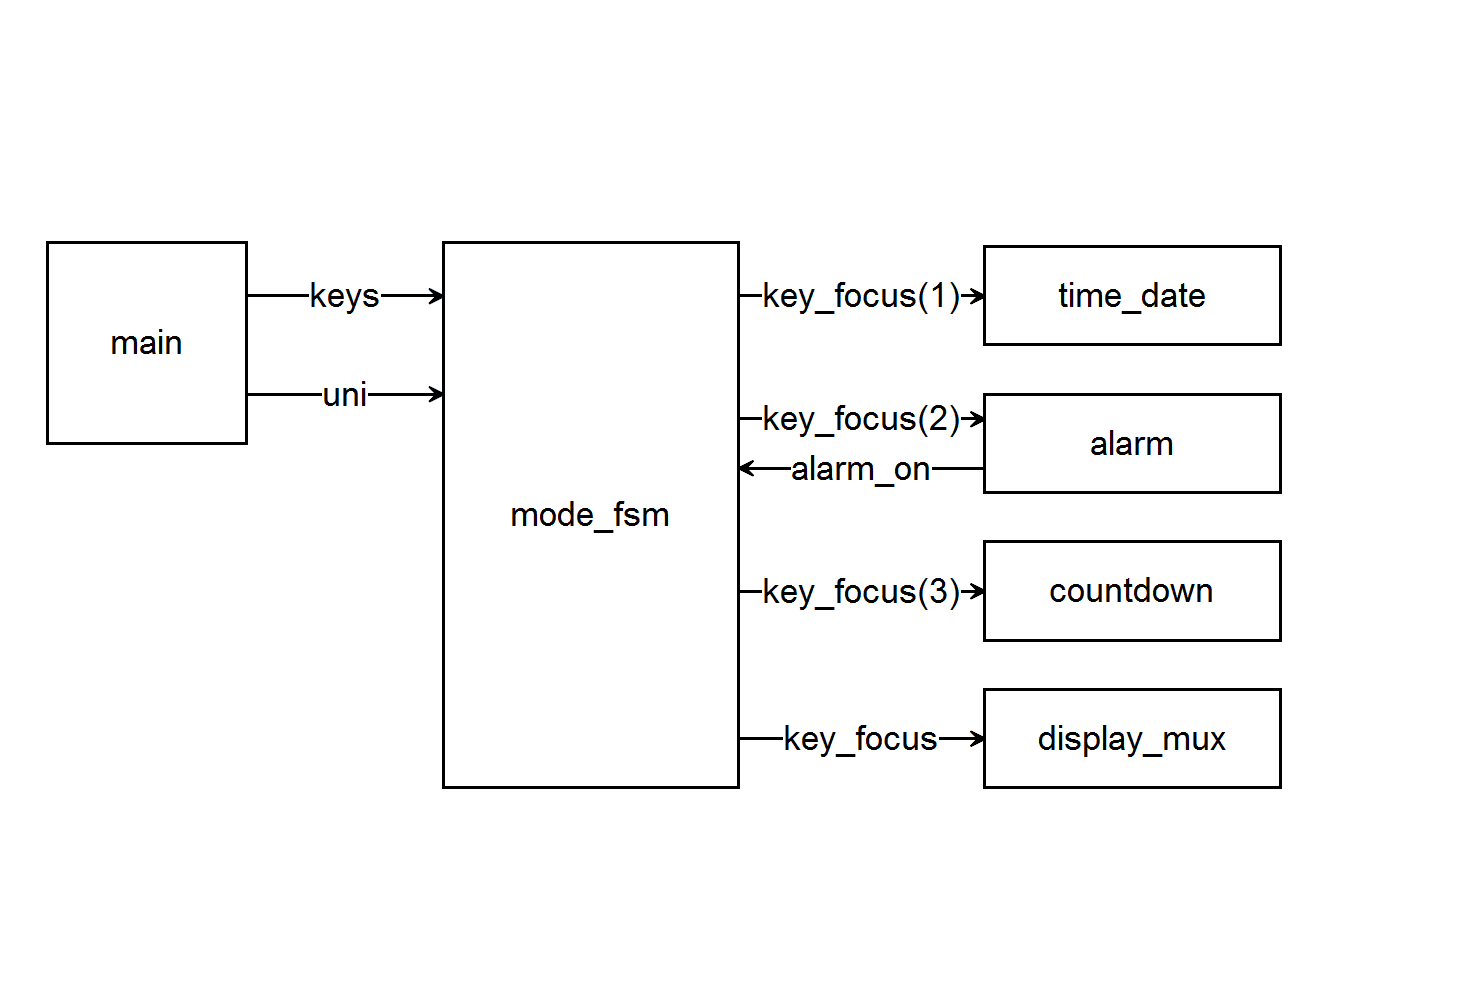
\includegraphics[width=100mm, height=70mm]{pictures/mode_fsm_interface.png}
  	\end{figure}
  \end{frame}
  
    \begin{frame}{Mode \_fsm Funktion}  
    	    \begin{itemize}
    	        \item Controls current mode
    	        \item Handles key access of modules (special case alarm ringing)
    	        \item Creates control signal for display\_mux
    	    \end {itemize}
    \end{frame}

  \begin{frame}{Mode \_fsm state diagram}
  	\begin{figure}
    	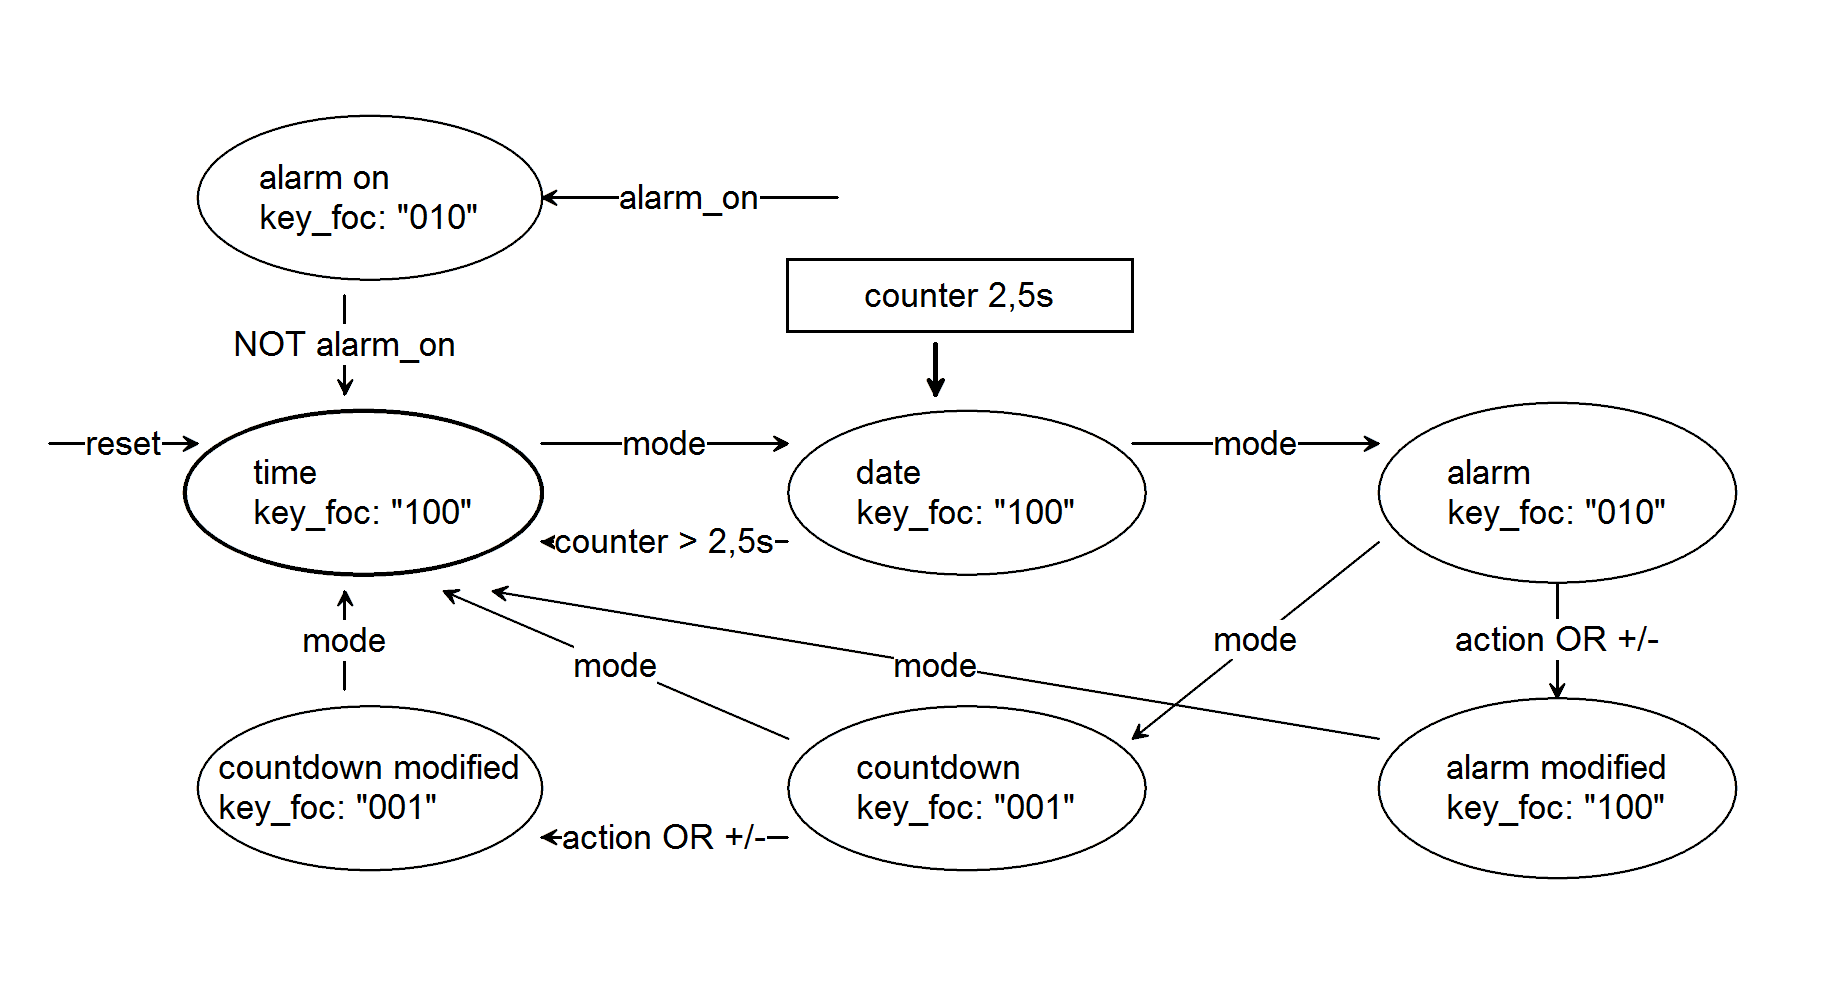
\includegraphics[width=100mm, height=70mm]{pictures/mode_fsm_state.png}
    \end{figure}
  \end{frame}



\section{Display MUX}
\begin{frame}{Display MUX Interface}
    \begin{columns}
    \begin{column}{6cm}
        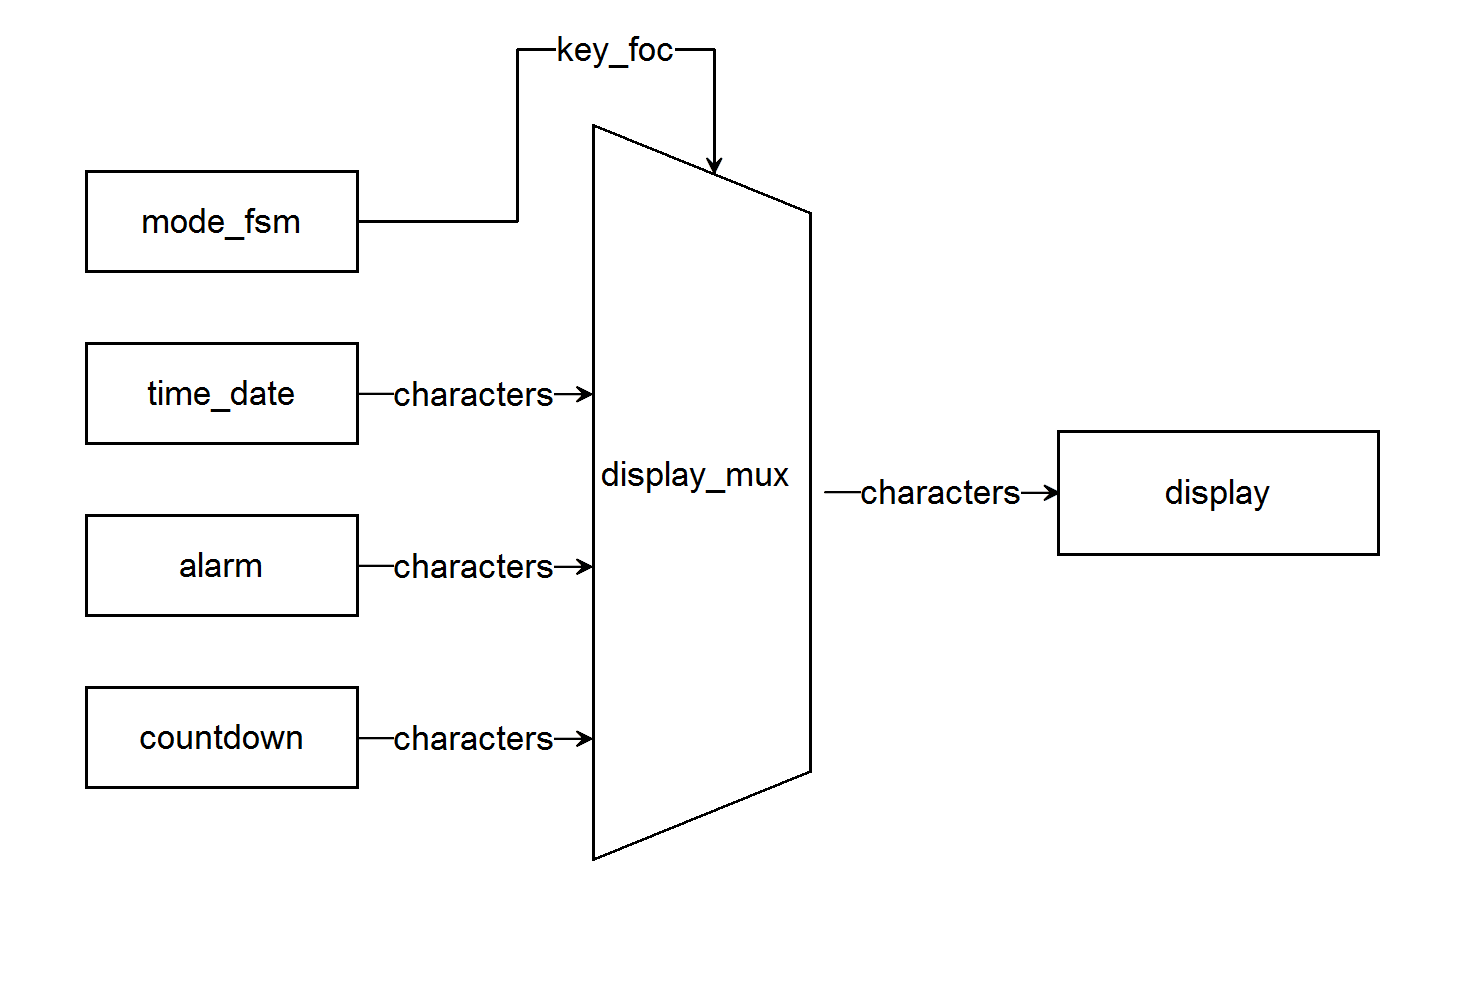
\includegraphics[width=60mm, height=50mm]{pictures/display_mux_interface.png}
    \end{column}
    \begin{column}{6cm}
    \begin{itemize}
        \item forwards characters of active module
        \item "DCF" string and star for active alarm always from time\_date/alarm module 
    \end {itemize}
    \end{column}
    \end{columns}
  \end{frame}
